\begin{frame}
        \titlepage
        \note[item]{Begrüßen. Bla Bla.}
        \note[item]{In diesem Vortrag mit dem Titel $\cdots$ fasse ich Thema und Zielsetzung meiner Masterarbeit bei Herrn Raasch kurz zusammen. Dabei kann das meiste nur oberflächlich behandelt werden. Weiter werden an entsprechenden Stellen Quellen angegeben, die das jeweilige Thema ausführlicher darstellen.}
        \note[item]{Zunächst wollen wir auf den Ursprung des Problems eingehen.}
\end{frame}

\begin{frame}[t]
    \frametitle{Overarching goal}
    We want to study the phase separation behavior of polymers.\footfullcite{Fredrickson:2006th}
    \vfill

    \begin{columns}
        \begin{column}{0.6\textwidth}
            \begin{itemize}
                \item<2-> \emph{polymers} are large molecules, composed of many repeated subunits (\emph{monomers})
                \item<2-> monomers interact with each other in and across polymers
                \item<2-> theory based on stochastic models (mainly \emph{ideal chain models})
                \item<3-> for simplicity, we consider only \emph{diblock copolymers}; linear chain polymers consisting of two types of monomers (e.g. A and B)
            \end{itemize}
        \end{column}
        \begin{column}{0.4\textwidth}
            \centering
            \onslide<2->
            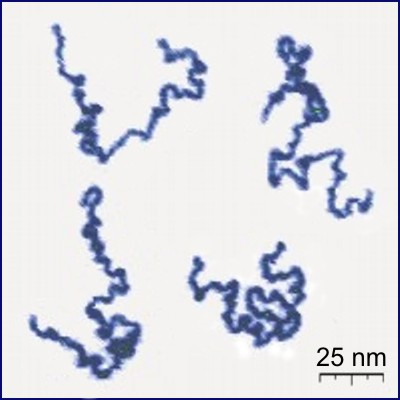
\includegraphics[width=0.9\textwidth]{figures/Single_Polymer_Chains_AFM.jpg}
        \end{column}
    \end{columns}
    \centering
    \onslide<3->
    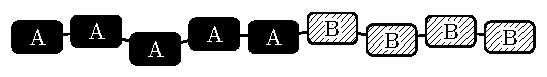
\includegraphics[width=0.8\textwidth]{figures/copoly2.pdf}
    \note[item]{Das Problem stammt aus der Polymerchemie und lässt sich kurz so zusammenfassen:}
    \note[item]{Wir wollen das Separationsverhalten von Polymeren untersuchen.}
    \note[item]{Bevor wir genauer darauf eingehen, wollen wir zunächst aber die Gegebenheiten klären:}
    \note[item]{Ein Polymer ist ein großes Molekül, das aus vielen, sich wiederholenden kleineren Bausteinen besteht. Diese werden Monomere genannt und stellen kleinere Moleküle dar.}
    \note[item]{Diese interagieren durch verschiedene Kräfte miteinander, sowohl in einem Polymer als auch zwischen Polymeren.}
    \note[item]{Theoretische Modelle von Polymeren stammen oft aus der Stochastik. Ein weit verbreitetes und relativ einfaches Modell ist das sogenannte Frei bewegliche Kettenmodell, bei dem ein Polymer im Grunde als Random Walk aufgefasst wird.}
    \note[item]{Diese haben eine nicht-atomistische Sicht; dies ist gerechtfertig, da Polymere meist aus mehreren dutzend / hundert Atomen bestehen.}
    \note[item]{Wir beschränken uns auf kettenförmige Diblock Copolymere, die aus zwei Monomer-Arten bestehen, die jeweils einen großen Block bilden.}
\end{frame}

\begin{frame}[t]
    \frametitle{Overarching goal}

    Polymer melts (liquid phase) can exhibit different separation behaviors:
    \begin{itemize}
        \item \emph{macrophase separation:} liquid-liquid separation (e.g. like water / oil); mostly seen in blends of different polymers.
        \item \emph{microphase separation:} distinct ordering of individual polymer chains.
    \end{itemize}

    \vfill

    \onslide<2->
    \begin{columns}
        \begin{column}{0.4\textwidth}
            Several types of microphase separation observable depending on the properties of the polymers, e.g. gyroid.
        \end{column}
        \begin{column}{0.5\textwidth}
            \centering
            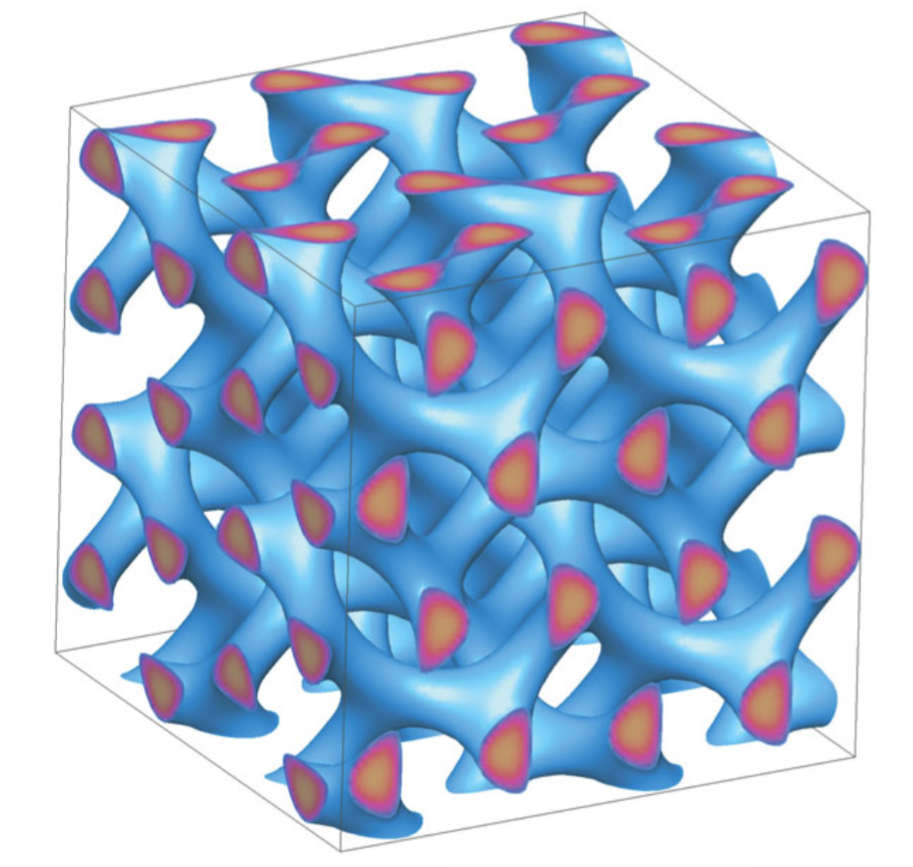
\includegraphics[width=0.9\textwidth]{figures/gyroid_separation.png}
        \end{column}
    \end{columns}
    %
    \note[item]{Der flüssige Aggregatszustand von Polymeren kann Separation auf zwei verschiedenen Skalen aufweisen.}
    \note[item]{Die makroskopische Separation, die meist bei Mischungen verschiedener Polymere beobachtet werden kann, verhält sich ähnlich wie die Mischung von Wasser und Öl. Man erhält getrennte Schichten.}
    \note[item]{Alterantiv gibt es auch die mikroskopische, diese kann oft bei Diblock Copolymeren beobachtet werden. Interaktion zwischen den A- und B-Blöcken verschiedener Polymerketten sorgen sorgen dafür, dass sich diese ebenfalls trennen wollen, dies kann aber nicht erfolgen, da diese ja Teil eines Polymers sind. Stattdessen ordnen sich die Polymerketten nach bestimmten Mustern an.}
    \note[item]{Es gibt verschiedene solche Muster.}
    \note[item]{Unser Ziel ist es nun, diese Anordnungen numerisch zu bestimmen.}
\end{frame}

\begin{frame}[t]
    \frametitle{So, what's self-consistent field theory?}
    Purpose of \emph{self-consistent field theory} (SCFT):
    \begin{itemize}
        \item Goal: study a complex stochastic model (e.g. a polymer melt) with a huge number of small interacting components (e.g. monomers).
        \item Idea: instead of considering interactions between all the individual components, approximate the effect on a given individual by a single averaged effect (so called \emph{external field}).
        \item<2-> \emph{This reduces a many-body problem to a one-body problem!}
    \end{itemize}

    \onslide<3->
    How can this be used?
    \begin{itemize}
        \item Model leads to a free energy functional depending on external fields $w_{A}$ and $w_{B}$, where \emph{saddle points} correspond to stable microphase separations.
        \item Allows an iterative scheme that adjusts the external fields until these satisfy some saddle point equations.
    \end{itemize}
    %\tabularnewline
    \note[item]{Wir können das stochastische Modell mit einer hohen Anzahl interagierender Teilchen nicht direkt untersuchen.}
    \note[item]{Hier kommt die selbstkonsistente Feldtheorie ins Spiel.}
    \note[item]{Diese ermöglicht die Untersuchung anhand eines vereinfachten Modells.}
    \note[item]{Dazu werden die Interaktionen zwischen den einzelnen Monomeren ersetzt durch ein externes Feld.}
    \note[item]{Dieses wird als Durchschnitt der auf ein einzelnes Teilchen wirkenden Kräfte gebildet und ignoriert Fluktuationen.}
    \note[item]{Damit wird ein Mehrkörperproblem auf ein Einkörperproblem reduziert.}
    \note[item]{Numerisch lässt sich das folgendermaßen nutzen: die Theorie führt zu einem Freie-Energie-Funktional, dessen Sattelpunkte gerade den stabilen Anordnungen entsprechen.}
    \note[item]{Das ganze kann dann als iteratives Verfahren zum Lösen der Sattelpunktgleichungen, die von den Feldern abhängen, aufgefasst werden.}
\end{frame}

\begin{frame}[t]
    \frametitle{So, what's self-consistent field theory?}

    Most costly part of each iteration: \emph{modified diffusion equation} (MDE)
        \begin{equation}
            \frac{\partial}{\partial s}q(\vec{r}, s) = c\,\Delta q(\vec{r}, s) - w(\vec{r}, s)q(\vec{r}, s), \quad q(\vec{r}, 0) = 1,
        \end{equation}
    where $c > 0$ and
    \onslide<2->
    \begin{itemize}
        \item the normalized polymer chain contour $s \in [0, 1]$,
        \item a position $\vec{r}$ in a small volume cell $\Omega \subset \mathbb{R}^{n}$ (bounded domain),
        \item the combined external field
        \begin{equation}
            w(\vec{r}, s) = \begin{cases}
                w_{A}(\vec{r}), & 1 \leq s < f \\
                w_{B}(\vec{r}), & f \leq s \leq 1
            \end{cases}
        \end{equation}
        with the ratio $f \in [0, 1]$ of $A$-type monomers in the polymer chain.
    \end{itemize}

    \onslide<3->
    Has to be solved \emph{several hundred / thousand times} with mostly slight variations in the external fields.
    %\tabularnewline
    \note[item]{In jeder Iteration muss dabei eine modifizierte Diffusionsgleichung, also eine parabolische partielle Differentialgleichung gelöst werden.}
    \note[item]{Diese hängt von den Feldern ab. Weiter werden diese Felder bei jeder Iteration angepasst. Das resultiert darin, dass man obige Differentialgleichung immer wieder für leicht verschiedene Felder lösen muss.}
\end{frame}

\begin{frame}[t]
    \frametitle{Example I}

    \begin{itemize}
        \item Let $\Omega = [0, 10]$ and $f = 1/2$.
        \item<2-> Final fields $w_A$, $w_B$ (using de facto default pseudospectral method\footfullcite{Stasiak:2011ba}).
        \item<3-> Corresponding Fourier coefficients (absolute value, in the order $\cos(2 \pi x), \sin(2 \pi x), \cos(4 \pi x), \dots$).
    \end{itemize}

    \begin{columns}
    \begin{column}{0.5\textwidth}
        \uncover<2->{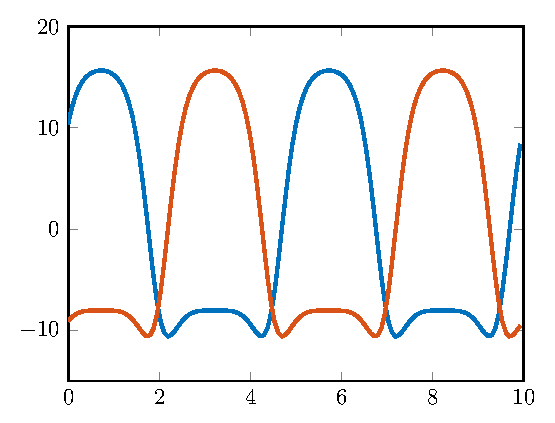
\includegraphics[width=\textwidth]{figures/scft1.pdf}}
    \end{column}
    \begin{column}{0.5\textwidth}
        \uncover<3->{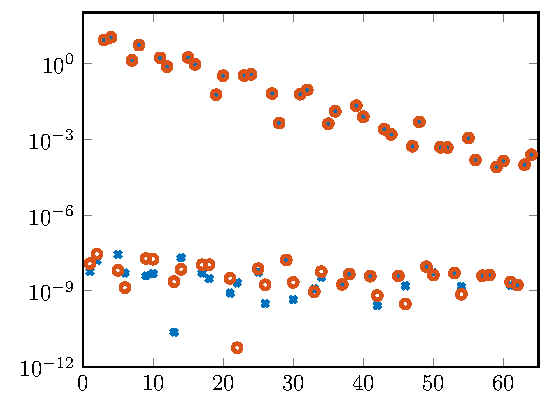
\includegraphics[width=\textwidth]{figures/scft2.pdf}}
    \end{column}
    \end{columns}
    \note[item]{Erstes Beispiel. Wir halten das meiste hier abstrakt, da es nur zur veranschaulichung dienen soll.}
    \note[item]{Auf der linken Seite sind die finalen Felder die mit der Pseudospektralmethode, die ein Standardverfahren dafür ist, bestimmt wurden.}
    \note[item]{Auf der rechten Seite sieht man die zugehörigen Fourier-Koeffizienten.}
    \note[item]{Die resultierenden Felder weisen Regularität und Symmetrien auf, ferner erkennt man auch, dass von den Fourierkoeffizienten viele nahezu null sind und die restlichen relativ schnell fallen.}
\end{frame}

\begin{frame}[t]
    \frametitle{Example II}

    And now the same with $f = 1/3$.

    \vfill
    \begin{columns}
    \begin{column}{0.5\textwidth}
        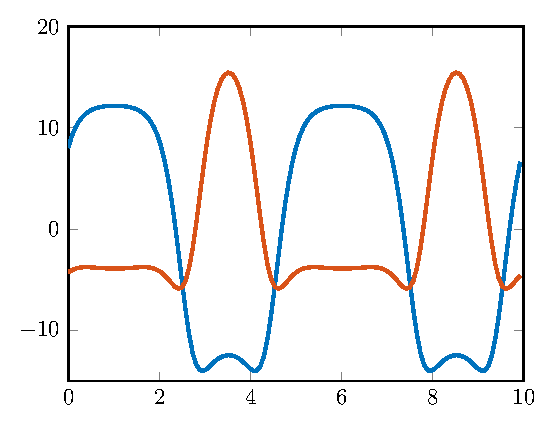
\includegraphics[width=\textwidth]{figures/scft_example2_fields.pdf}
    \end{column}
    \begin{column}{0.5\textwidth}
        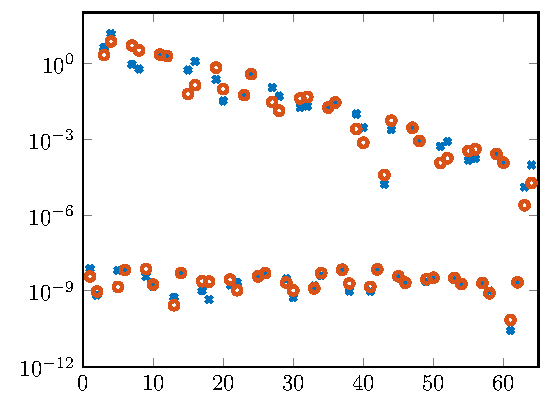
\includegraphics[width=\textwidth]{figures/scft_example2_fourier_coeffs.pdf}
    \end{column}
    \end{columns}
    \vfill
    \onslide<2->
    Maybe a good leverage point for model reduction by only considering the functions with significant coefficients\\
    $\rightarrow$ model reduction by \emph{reduced basis method}.
    %\tabularnewline
    \note[item]{Zweites Beispiel mit leicht anderen Daten. Hier sind ähnliche Ergebnisse zu sehen.}
    \note[item]{Eventuell ist damit ein guter Ansatzpunkt für eine Modellreduktion gegeben. Wir entwickeln die Felder in einem geeigneten Funktionensystem und betrachten dann nur die signifikanten Koeffizienten. Dies würde dann die Anwendung einer Reduzierte-Basis-Methode erlauben. Diese wollen wir jetzt kurz noch einmal wiederholen und beschreiben, wie wir diese umgesetzt haben.}
\end{frame}

\begin{frame}[t]
    \frametitle{Intermission: Reduced Basis Method\footfullcite{Quarteroni2016}}
    \framesubtitle{Preliminaries}

    Given a \emph{parametric variational problem}
    \begin{equation}
        b(u, v; \bm \sigma) = f(v; \bm \sigma), \qquad u \in \mathcal X,~v \in \mathcal Y,
    \end{equation}\\[-1em]
    \begin{itemize}
        \item $\mathcal X, \mathcal Y$ are Hilbert spaces,
        \item $\mathcal P \subset \mathbb{R}^{P}$, $P \in \mathbb{N}$, is a closed parameter space,
        \item $b \colon \mathcal X \times \mathcal Y \times \mathcal P \to \mathbb{R}$ is a parametric continuous bilinear form,
        \item $f \colon \mathcal Y \times \mathcal P \to \mathbb{R}$ is a parametric continuous linear functional.
        \item<2-> Assume
        \begin{equation}
            \beta(\bm \sigma) := \infsup{u \in \mathcal X}{v \in \mathcal Y} \frac{b(u, v; \bm \sigma)}{\norm{u}_{\mathcal X}\norm{v}_{\mathcal Y}}  > 0 \qquad \text{for all } \bm \sigma \in \mathcal P.
        \end{equation}
        $+$ some minor assumptions $\Rightarrow$ for every $\bm \sigma \in \mathcal P$ exists a unique solution $u(\bm \sigma)$.
    \end{itemize}
    \note[item]{Um die RBM zu erklären, müssen wir zunächst geeignete Rahmenbedingungen schaffen. Dies machen wir durch einführen eines abstrakten parametrischen Variationsproblems.}
    \note[item]{Weiter treffen wir eine wichtige Annahme, die uns garantiert, dass das vorliegende Variationsproblem zu jedem Parameter eine eindeutige Lösung besitzt.}
\end{frame}

\begin{frame}[t]
    \frametitle{Intermission: Reduced Basis Method}
    \framesubtitle{Basic idea}

    \onslide
    Assume we want to compute the solution $\bm \sigma \mapsto u(\bm \sigma)$ in real time or for lots of different parameters $\bm \sigma \in \mathcal P$\\
    $\rightarrow$ standard Galerkin methods are likely too slow!

    \begin{itemize}
        \item \onslide<2->Let $\mathcal M := \Set{ u(\bm \sigma) \given \bm \sigma \in \mathcal P }$.
        \item Depending on the properties of the variational problem, $\mathcal M$ is often a \emph{smooth manifold with low dimension}.
        \item This can be used for model reduction: instead of $\mathcal X$ use $\mathcal M$ as the ansatz space!
    \end{itemize}

    \vfill

    \onslide<3->
    Further we won't use the continuous variational problem, but instead the \emph{truth variational problem} based on a high dimensional Galerkin method:
    \begin{equation}
        b(u, v; \bm \sigma) = f(v; \bm \sigma), \qquad u \in \mathcal X_{\mathcal N}, v \in \mathcal Y_{\mathcal N},
    \end{equation}
    with subspaces $\mathcal X_{\mathcal N} \subset \mathcal X$, $\mathcal Y_{\mathcal N} \subset \mathcal Y$.
    \note[item]{Wir betrachten das folgende Problem: wir wollen das parametrische Variationsproblem in Echtzeit oder für viele verschiedene Parameter lösen. Wollen wir das mit zufriedenstellender Genauigkeit, dann sind Standardverfahen wie biepielsweise Galerkin verfahren zu langsam.}
    \note[item]{Wie kann man das ganze mittels Modellreduktion beschleunigen?}
    \note[item]{Wir betrachten die parametrische Lösungsmenge. Diese ist, je nach Eigenschaften des Variationsproblems, oftmals eine niedrigdimensionale Mannigfaltigkeit. Da sie weiter alle Lösungen enthält, können wir diese statt dem eigentlichen Ansatzraum verwenden.}
    \note[item]{Das ist die zugrundeliegende Idee hinter der Reduzierte-Basis-Methode.}
    \note[item]{Diese geht weiter nicht vom eigentlichen Variationsproblem aus, sondern baut auf eine hochdimensionale Galerkin-Diskretisierung auf. Diese werden wir im weiteren als Truth-Variationsproblem bezeichnen.}
\end{frame}

\begin{frame}[t]
    \frametitle{Intermission: Reduced Basis Method}
    \framesubtitle{Basic idea}

    The reduced basis method consists of two stages:

    \begin{itemize}
        \item \onslide<2-> \emph{Offline stage:} Construction of \enquote{optimal} reduced basis spaces $\mathcal X_{N} := \Set{u_{\mathcal N}(\bm \sigma_n) \given n = 1, \dots, N} \subset \mathcal M_{\mathcal N}$ and $\mathcal Y_{N} \subset \mathcal Y_{\mathcal N}$ with low dimension $N \ll \mathcal N$.
        \item \onslide<3-> \emph{Online stage:} Given a parameter $\bm \sigma \in \mathcal P$, compute the rb-solution $u_{N}(\bm \sigma)$ and a certified bound for the error $\norm{u_{N}(\bm \sigma) - u_{\mathcal N}(\bm \sigma)}_{\mathcal X}$ \\(both independent of $\mathcal N$).
    \end{itemize}
    \centering
    $\;$\\[-3.7em]
    \onslide<2-> 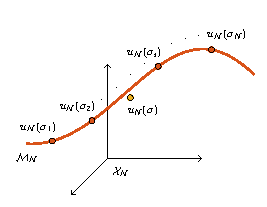
\includegraphics[width=0.58\textwidth]{figures/rb.pdf}
    %\tabularnewline
    \note[item]{Die Reduzierte-Basis-Methode ist im Grunde ein weiteres Galerkin-Verfahren und lässt sich in zwei Phasen einteilen, die auch gleichzeitig eine effektive Berechnung ermöglichen.}
    \note[item]{In der Offline-Phase werden die niedrigdimensionalen Reduzierte-Basis-Räume optimal konstruiert. Dazu werden einige Parameter zielgerichtet aus dem Parameterraum ausgewählt und für diese werden mittels Truth-Verfahren die Lösung bestimmt. Diese Lösungen werden als Basis für ein weiteres Galerkin-Verfahren verwendet.}
    \note[item]{Ziel bei der Parameterauswahl ist die Reduktion des Fehlers über alle Parameter.}
    \note[item]{In der Online-Phase werden dann die Reduzierte-Basis-Lösung und eine zertifizierte Schranke für den Fehler berechnet.}
\end{frame}

\begin{frame}[t]
    \frametitle{Intermission: Reduced Basis Method}
    \framesubtitle{Certified error bound}
    Let $r_{N} \colon \mathcal Y_{\mathcal N} \times \mathcal P \to \mathbb{R}$ be the \emph{residual}
    \begin{equation}
        r_{N}(v; \bm \sigma) := b(u_{\mathcal N}(\bm \sigma) - u_{N}(\bm \sigma), v; \bm \sigma) = f(v; \bm \sigma) - b(u_{N}(\bm \sigma), v; \bm \sigma).
    \end{equation}
    $\Rightarrow$ continuous linear functional for every $\bm \sigma \in \mathcal P$.

    \onslide<2>
    Standard theorems lead to \emph{a posteriori error bound}
    \begin{equation}
        \norm{u_{N}(\bm \sigma) - u_{\mathcal N}(\bm \sigma)}_{\mathcal X} \leq \frac{\norm{r_{N}(\blank; \bm \sigma)}_{\mathcal Y_{\mathcal N}'}}{\beta_{\mathrm{LB}}(\bm \sigma)} =: \Delta_{N}(\bm \sigma),
    \end{equation}
    where
    \begin{itemize}
        \item the norm of the residual can be efficiently computed through the Riesz representation theorem,
        \item $\beta_{\mathrm{LB}}(\bm \sigma)$ is a computable lower bound for $\beta(\bm \sigma)$.
    \end{itemize}
    \note[item]{Als wichtiger Teil der Reduzierte-Basis-Methode ist eine effizient berechnebare obere Schranke für den Fehler. Dieser wird über das folgende Residuum hergeleitet.}
    \note[item]{Es lässt sich zeigen, dass das Residuum ein stetiges lineares Funktional ist und damit erhält man mit Standard-Sätzen die folgende Abschätzung.}
    \note[item]{Diese lässt sich wegen obiger Form des Residuums als a posteriori Fehlerabschätzung verwenden.}
\end{frame}

\begin{frame}[t]
    \frametitle{Intermission: Reduced Basis Method}
    \framesubtitle{Inf-sup-constant}

    Problem: how to compute $\beta_{\mathrm{LB}}(\bm \sigma)$ efficiently?

    \vfill
    \onslide<2->
    Default: \emph{successive constraint method}\footfullcite{Huynh2007}.

    \begin{itemize}
        \item Reinterpret the calculation of $\beta(\bm \sigma)$ as an optimization problem
        \\$\rightarrow$ linear objective function, but feasible region in general not a convex polytope.
        \item \onslide<3->\emph{Offline stage:} Construct \enquote{optimal} lower and upper bounds for the feasible region.
        \item \emph{Online stage:} Compute $\beta_{\mathrm{LB}}(\bm \sigma)$ through small linear program.
    \end{itemize}

    \vfill
    \note[item]{Dazu muss die inf sup Konstante für einen Parameter schnell ausgewertet werden können. Exakte Bestimmung ist in Form eines Eigenwertproblems möglich, aber viel zu langsam.}
    \note[item]{Die Standard-Methode bei der Reduzierte-Basis-Methode ist die Successive Constraint Method.}
    \note[item]{Dabei wird die Bestimmung der parametrischen inf-sup-Konstante als Optimierungsproblem mit linearer Zielfunktion aufgefasst.}
    \note[item]{Der zulässige Bereich ist kein konvexes Polytop. Ziel ist, eine Ober- und eine Untermenge zu konstruieren und diese als zulässigen Bereich für ein lineares Optimierungsproblem zu verwenden.}
\end{frame}

\begin{frame}[t]
    \frametitle{Intermission: Reduced Basis Method}
    \framesubtitle{Offline and online stage}

    Offline stage of RBM needs a discrete \enquote{training set} $\mathcal P_{\mathrm{train}} \subset \mathcal P$.\newline
    \emph{Iterative greedy scheme}, start with random $\bm \sigma_{1} \in \mathcal P_{\mathrm{train}}$, $\mathcal X_{1} := \Set{u_{\mathcal N}(\bm \sigma_{1})}$:\\[0em]
    \begin{enumerate}
        \item find $\bm \sigma_{N + 1} := \argmax_{\bm \sigma \in \mathcal P_{\mathrm{train}}} \Delta_{N}(\bm \sigma)$,
        \item set $\mathcal X_{N + 1} := \spn (\mathcal X_{N} \cup \Set{u_{\mathcal N}(\bm \sigma_{N + 1})})$,
        \item repeat until maximum in step 1 is smaller than a given tolerance.
    \end{enumerate}
    $\rightarrow$ computationally intensive part.
    \vfill

    \onslide<2->
    Online stage, given a $\bm \sigma \in \mathcal P$:\\[0em]
    \begin{enumerate}
        \item solve reduced basis system for $u_{N}(\bm \sigma) \in \mathcal X_{N}$,
        \item compute certified error bound $\Delta_{N}(\bm \sigma)$.
    \end{enumerate}
    \emph{$\rightarrow$ runtime depends only on low dimension $N$, not $\mathcal N$}.
    %
    \note[item]{Damit kann die eigentliche Reduzierte-Basis-Methode beschrieben werden.}
    \note[item]{In der Offline-Phase können die Reduzierte-Basis-Räume mittels Greedy-Iterationsverfahren konstruiert werden. Dabei wird in jedem Iterationsschritt der Parameter bestimmt, der den a posteriori Fehlerschätzer maximiert.}
    \note[item]{Das Verfahren wird so lange wiederholt, bis der Fehler unter einer Toleranz liegt.}
    \note[item]{In der Online-Phase kann dann für einen gegebenen Parameter ein niedrigdimensionales System gelöst werden und weiter der a posteriori Fehlerschätzer bestimmt werden.}
    \note[item]{Das ganze kann unabhängig von der Dimension des Truth-Verfahrens getan werden!}
\end{frame}

\begin{frame}[t]
    \frametitle{Intermission: Reduced Basis Method}
    \framesubtitle{Examples}

    Typical results of the offline stage, one dimensional parameter space.

    \centering
    \includegraphics<1>[width=0.9\textwidth]{figures/1d_par_s_1.pdf}
    \includegraphics<2>[width=0.9\textwidth]{figures/1d_par_s_2.pdf}
    \includegraphics<3>[width=0.9\textwidth]{figures/1d_par_s_3.pdf}
    \includegraphics<4>[width=0.9\textwidth]{figures/1d_par_s_4.pdf}
\end{frame}

\begin{frame}[t]
    \frametitle{Intermission: Reduced Basis Method}
    \framesubtitle{Examples}

    And now a four dimensional parameter space.

    \centering
    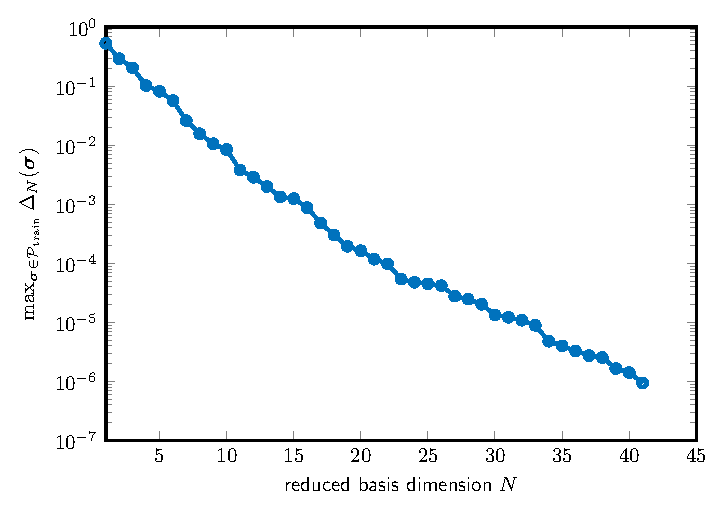
\includegraphics[width=0.9\textwidth]{figures/ch5ex2_rbm_error.pdf}
\end{frame}


\begin{frame}[t]
    \frametitle{Back to the SCFT}

    What we've already done:

    \begin{itemize}
        \item<1-> Derived a \emph{space-time variational formulation} (STVP) of the MDE based on \emph{Bochner spaces}; showed \emph{well-posedness}.
        \item<2-> Replaced the fields $w_A, w_B$ with parametric functions
        \begin{equation}
            w(\bm \sigma) = \sum_{j = 1}^{N} \sigma_{j} \phi_{j},
        \end{equation}
        where $N \in \mathbb{N} \cup \Set{ \infty }$, $\bm \sigma \in [-1, 1]^{N}$ and $\phi_{j} \in L_{\infty}(\Omega)$, $j = 1, \dots, N$.
        \item<2-> Shown that the solution of the STVP depends \emph{analytically} on the parameters (given some restrictive sufficient conditions).
        \item<3-> Applied a \emph{Petrov-Galerkin} method to solve the STVP.
        \item<3-> Experimented with the application of the reduced basis method on the STVP.
    \end{itemize}

    \note[item]{So viel zur Reduzierte-Basis-Methode. Jetzt kehren wir kurz zur selbstkonsistenten Feldtheorie zurück und zeigen auf, was im Rahmen meiner Masterarbeit getan wurde.}
    \note[item]{Zunächst haben wir eine Raum-Zeit-Variationsformulierung der MDE basierend auf Bocher-Räumen hergeleitet.}
    \note[item]{Weiter haben wir die verwendeten Felder durch Reihenentwicklungen ersetzt und die Entwicklungskoeffizienten als Parameter aufgefasst.}
    \note[item]{Für diese parametrischen Variationsprobleme haben wir dann gezeigt, dass die Lösung unter gewissen hinreichenden, leider etwas einschränkenden Bedingungen, analytisch vom Parameter abhängt. Das ist für die Reduzierte-Basis-Methode nicht notwendig, aber trotzdem ein gutes Ergebnis.}
    \note[item]{Dann haben wir als Truth-Verfahren eine Petrov-Galerkin-Diskretisierung drauf angewandt.}
    \note[item]{Und zuletzt mit der beschriebenen Reduzierte-Basis-Methode rumexperimtentiert.}
\end{frame}

\begin{frame}[t]
    \frametitle{Back to the SCFT}

    Problems encountered so far:

    \begin{itemize}
        \item<1-> The fact that $\mathcal X \neq \mathcal Y$ complicates lots of things.
        \item<2-> Most suitable Petrov-Galerkin methods aren't unconditionally stable.
        \item<3-> Successive constraint method suffers from curse of dimensionality and is quite slow for more than a handful of parameters.
        \\ $\rightarrow$ a priori knowledge about field expansion functions required to reduce number of parameters.
    \end{itemize}

    \note[item]{Dabei sind unter anderem folgende Probleme aufgetaucht, die wir hier zusammenfassen.}
    \note[item]{Die Tatsache, dass Ansatz und Testraum ungleich sind, macht einiges schwer. Symmetrische und vor allem koerzive Variationsprobleme sind deutlich angenehmer.}
    \note[item]{Petrov-Galerkin Verfahen sind im allgemeinen nicht bedingungslos stabil. In unserem Fall führt es zu einer CFL-artigen Bedingung, die man bei dem Verfahren auch nicht loswird.}
    \note[item]{Vielleicht gibt es da besser geeignete Verfahren.}
    \note[item]{Weiter ist die SCM nur bedingt geeignet. Theoretisch brauchbar, leidet sie in der Praxis bei mehr als einer handvoll Parameter massiv unter dem Fluch der Dimensionalität und wird mit jeder Parameterdimension sehr viel langsamer.}
\end{frame}
